\documentclass{beamer}
\usepackage{basileabeam}
\usepackage{array}% http://ctan.org/pkg/
\usepackage[math]{cellspace}
\usepackage{textcomp} % to write the degre sign: °
\usepackage{varwidth}
\usepackage{booktabs}% http://ctan.org/pkg/booktabs
\usepackage{transparent}
%\usepackage{paralist}
\usepackage{pgfplots}
\pgfplotsset{width=11cm, height=6.5cm,compat=1.9}
\usepackage{tikz}
\usetikzlibrary{decorations.pathmorphing}
\usetikzlibrary{decorations.markings}
\usetikzlibrary{arrows.meta,bending}
\usetikzlibrary{shapes,arrows,chains}
\usetikzlibrary[calc]
\usetikzlibrary{decorations.text}
\usepackage{graphicx,caption}
\usepackage{tabularx,array,booktabs}
\renewcommand{\tabularxcolumn}[1]{m{#1}}
\newcommand{\tabitem}{~~\llap{\textbullet}~~}
\AtBeginEnvironment{figure}{\setcounter{subfigure}{0}}% Resets subfigure counter at start of figure environment
\setlength{\extrarowheight}{2pt}
%notes
%\pgfpagesuselayout{2 on 1}[a4paper,border shrink=5mm]
%\setbeamertemplate{note page}[plain]
%\setbeameroption{show notes on second screen=bottom}
\pgfkeys{
	/pgf/number format/precision=0, 
	/pgf/number format/fixed zerofill=true
}


\title              {An Empirical Comparison of Deep Learning and 3DMM-Based Approaches for Facial Occlusion Segmentation}

\author             {Elias Arnold}
\email              {elias.arnold@stud.unibas.ch}
\institute          {Department of Mathematics and Computer Science, University of Basel}

\date               {10.08.2018}

\ulogo        		{Template/header}
\ulistelement    	{Template/listelement}

\graphicspath{{Figures/}}
\usepackage{subfig}
\setlength{\fboxsep}{0pt}


\begin{document}
		
\begin{frame}[t,plain]
\titlepage
\end{frame}


\begin{frame}[c]{Overview}
	\begin{itemize}
		\item Motivation
		\item Occlusion Segmenation with an FCN
		\item Experiment: Segmentation Quality
		\begin{itemize}
			\item Qualitative segmenation results
			\item Quantitative segmentation results
		\end{itemize}
		\item Experiment: Fitting under occlusion
		\item Application to real-life data and conclusion
		\item Future Work
	\end{itemize}
\end{frame}


\begin{frame}[c]{The Goal}
	\begin{figure}
		\centering
		\subfloat[original]{\fbox{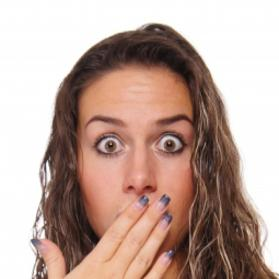
\includegraphics[width=.26\linewidth]{example/original.png}}}\qquad
		\subfloat[mask]{\fbox{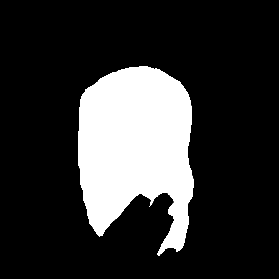
\includegraphics[width=.26\linewidth]{example/GROTRU_mask.png}}}\qquad
		\subfloat[resulting fit]{\fbox{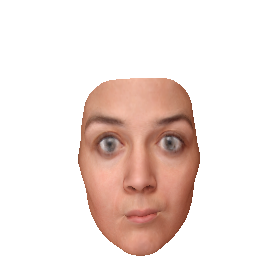
\includegraphics[width=.26\linewidth]{example/fit_GROTRU.png}}}
		\caption{Fitting with a perfect mask}
		\label{fig:1}
	\end{figure}
\end{frame}


\begin{frame}[c]{The Problem (Segmentation under Occlusion)}
	\begin{figure}
		\centering
		\subfloat[original]{\fbox{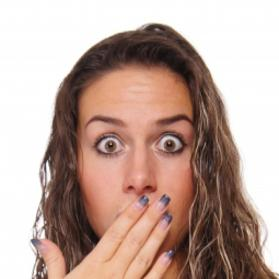
\includegraphics[width=.39\linewidth]{example/original.png}}}\qquad
		%\subfloat[mask]{\fbox{
\includegraphics[width=.26\linewidth]{example/DUMMY.png}}}\qquad
		\subfloat[resulting fit]{\fbox{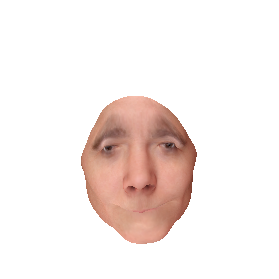
\includegraphics[width=.38\linewidth]{example/fit_DUMMY.png}}}
		\caption{Fitting without a mask}
		\label{fig:2}
	\end{figure}
\end{frame}

%\begin{frame}[c]{The Problem (segmentation under occlusion)}
%	\begin{figure}
%		\centering
%		\subfloat[original]{\fbox{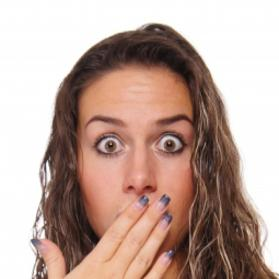
\includegraphics[width=.26\linewidth]{example/original.png}}}\qquad
%		\subfloat[mask]{\fbox{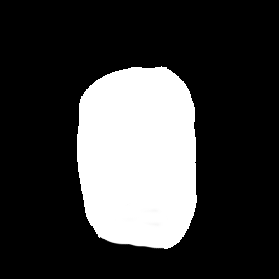
\includegraphics[width=.26\linewidth]{example/FULLFACE.png}}}\qquad
%		\subfloat[resulting fit]{\fbox{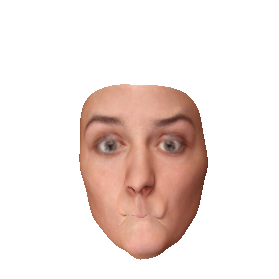
\includegraphics[width=.26\linewidth]{example/fit_FULLFACE.png}}}
%		\caption{fitting on the facial region only}
%		\label{fig:2}
%	\end{figure}
%\end{frame}

\begin{frame}[c]{Overview}
	\begin{itemize}
		\item \texttransparent{0.4}{Motivation}
		\item Occlusion Segmenation with an FCN
		\item \texttransparent{0.4}{Experiment: Segmentation Quality}
		\begin{itemize}
			\item \texttransparent{0.4}{Qualitative segmenation results}
			\item \texttransparent{0.4}{Quantitative segmentation results}
		\end{itemize}
		\item \texttransparent{0.4}{Experiment: Fitting under occlusion}
		\item \texttransparent{0.4}{Application to real-life data and conclusion}
		\item \texttransparent{0.4}{Future Work}
	\end{itemize}
\end{frame}

\begin{frame}[c]{Convolutional Neural Network (CNN)}
	%\begin{columns}
		%\column{.5\textwidth}
		\begin{itemize}
			\item Artificial Neural Network
			\item fully connected layers at the end
			\item makes decisions based on global information
		\end{itemize}
		%\column{.5\textwidth}
		
		\begin{figure}
			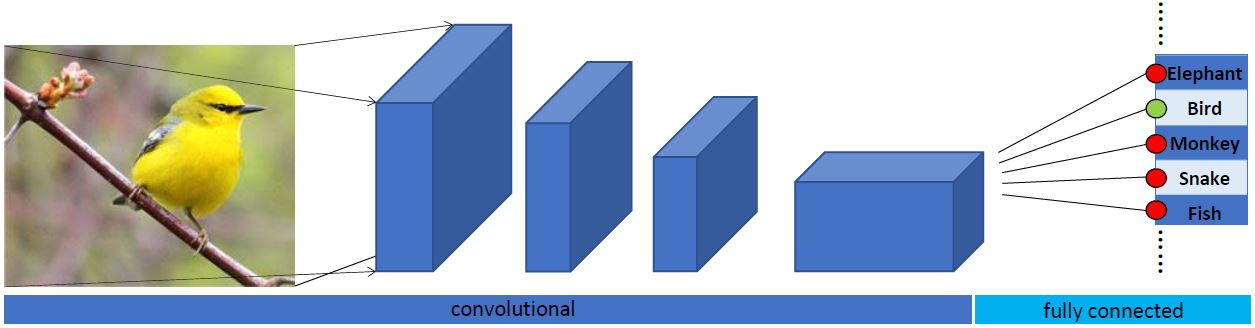
\includegraphics[width=1\textwidth]{intro/classicalCNN.JPG}
			\caption{A classical neural network}
		\end{figure}
	%\end{columns}
\end{frame}

\begin{frame}[c]{Fully Convolutional Network (FCN)}
	%\begin{columns}
	%\column{.5\textwidth}
	\begin{itemize}
		\item without fully connected layers at the end
		\item makes decisions based on spatial information
	\end{itemize}
	%\column{.5\textwidth}
	
	\begin{figure}
		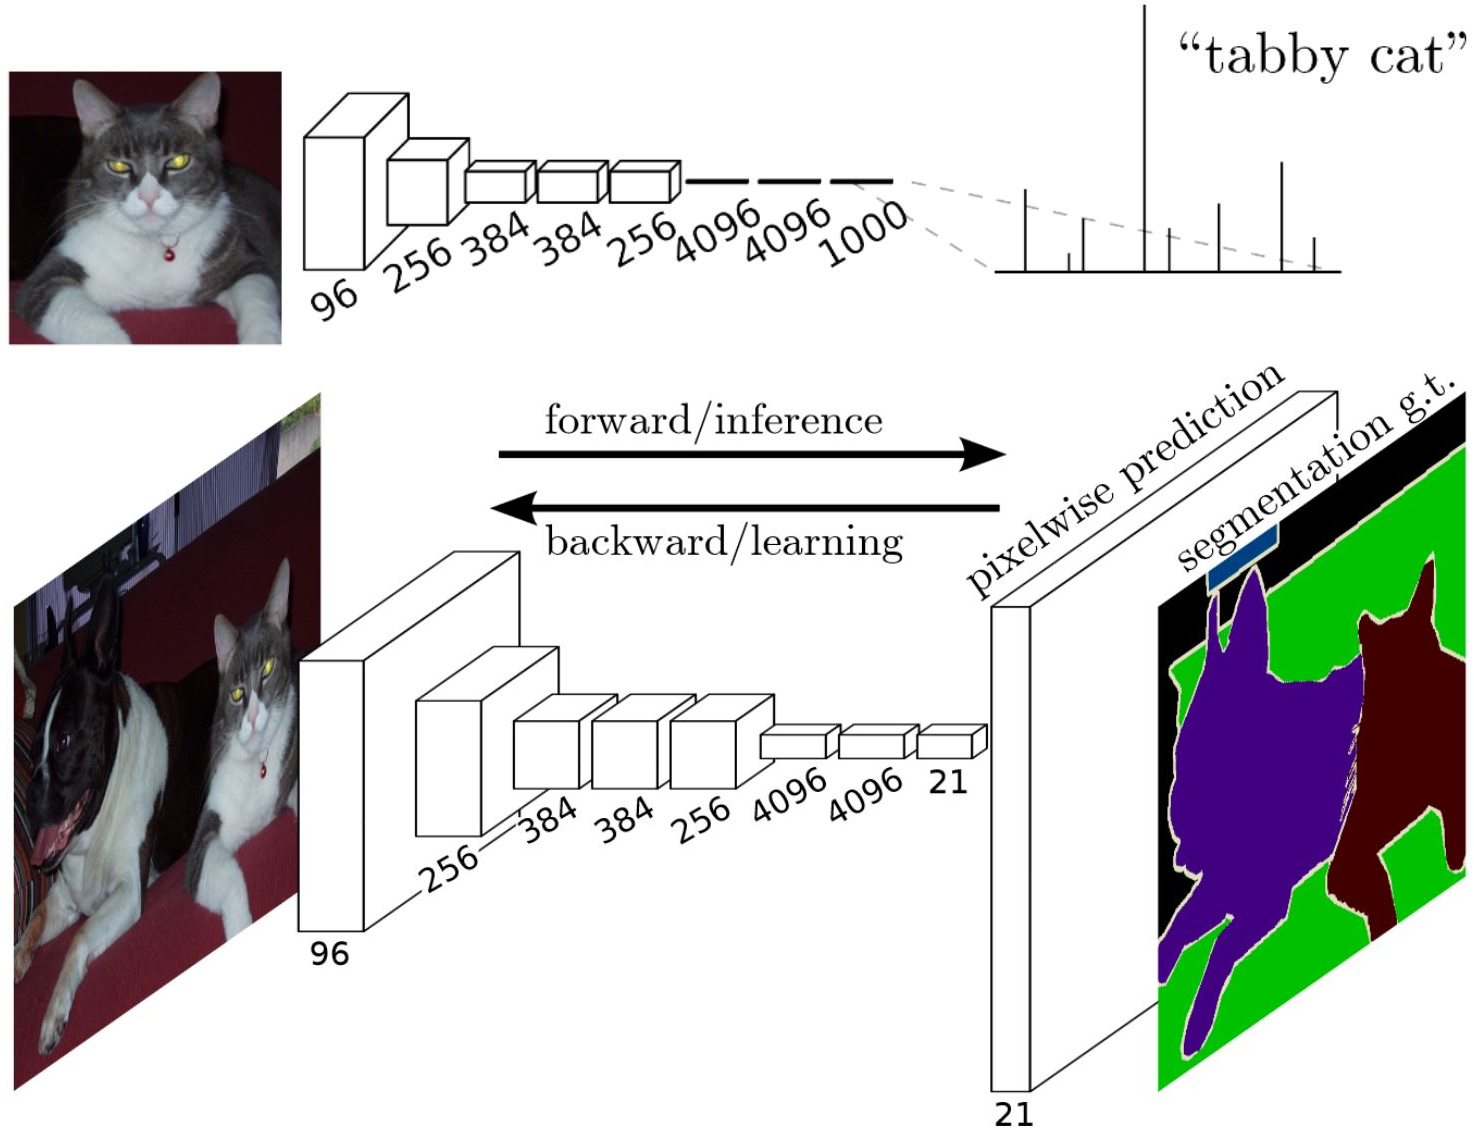
\includegraphics[width=0.65\textwidth]{intro/jlong.png}
		\caption{The transformation from a CNN into a FCN}
	\end{figure}
	%\end{columns}
\end{frame}

\begin{frame}[c]{Training of the FCN}
	\begin{itemize}
		\item The FCN was trained by Nirkin et al.
		\item They used the well known FCN-8s-VGG network
		\item Training Data: Frames of Videos
		\item Frame used multiple times (synthetic occlusions)
		\item Total: 9'818 facial images
	\end{itemize}
	\begin{figure}
		\centering
		\subfloat{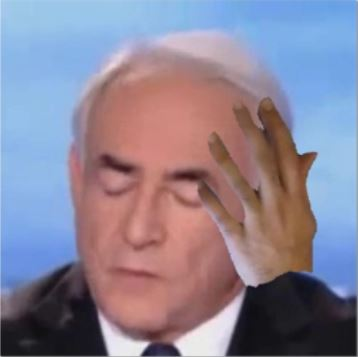
\includegraphics[width=.3\linewidth]{Bilder_Praesentation/TestFrame_1.JPG}}\qquad
		\subfloat{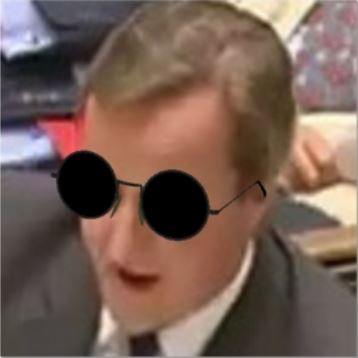
\includegraphics[width=.3\linewidth]{Bilder_Praesentation/TestFrame_2.JPG}}
		\caption{Two images used for training. They are overlaid them with an synthetic occlusion.}
	\end{figure}
\end{frame}


\begin{frame}[c]{Overview}
	\begin{itemize}
		\item \texttransparent{0.4}{Motivation}
		\item \texttransparent{0.4}{Occlusion Segmenation with an FCN}
		\item Experiment: Segmentation Quality
		\begin{itemize}
			\item Qualitative segmenation results
			\item \texttransparent{0.4}{Quantitative segmentation results}
		\end{itemize}
		\item \texttransparent{0.4}{Experiment: Fitting under occlusion}
		\item \texttransparent{0.4}{Application to real-life data and conclusion}
		\item \texttransparent{0.4}{Future Work}
	\end{itemize}
\end{frame}

\begin{frame}[c]{Qualitative Evaluation on the COFW Dataset}
	\begin{itemize}
		\item \textbf{C}altech \textbf{O}ccluded \textbf{F}aces in the \textbf{W}ild
		\item used of Nirkin et al themselves
	\end{itemize}
	\begin{figure}
		\centering
		\subfloat[Six segmentations of the FCN]{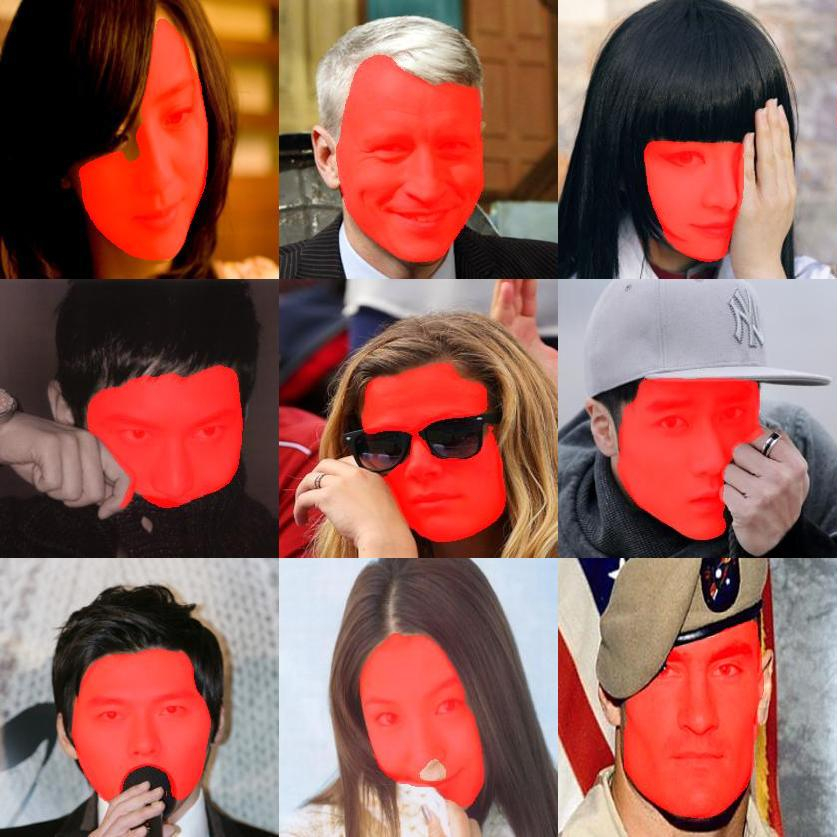
\includegraphics[width=.45\linewidth]{myMatrix.jpg}}\quad
		\subfloat[Six segmentations of the approach of Egger et al]{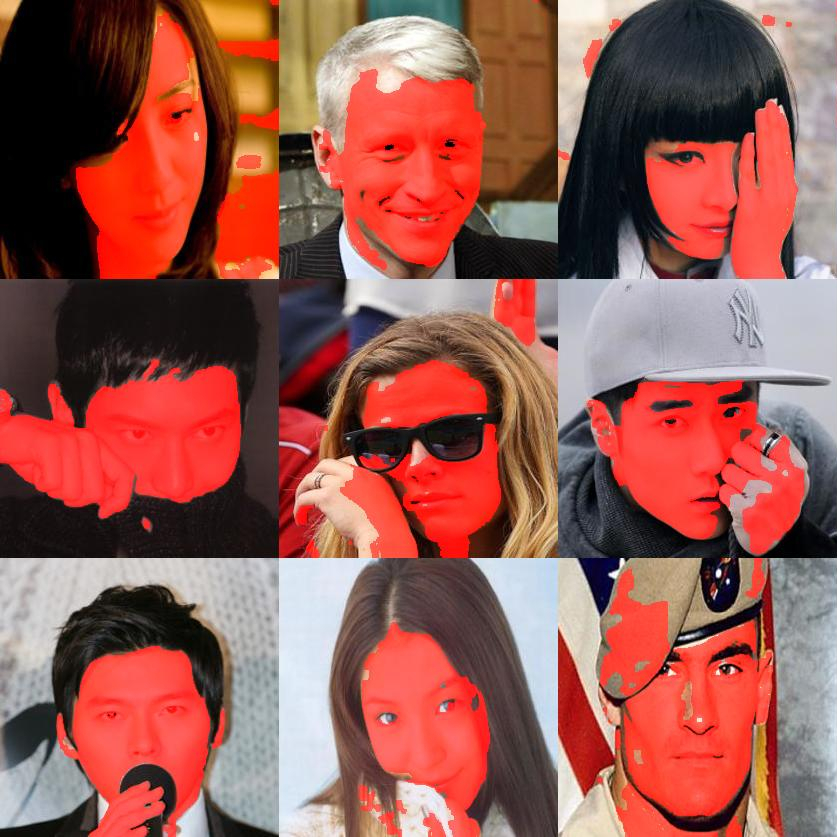
\includegraphics[width=.45\linewidth]{myMatrix_EGGER.jpg}}
	\end{figure}
\end{frame}

\begin{frame}[c]{Overview}
	\begin{itemize}
		\item \texttransparent{0.4}{Motivation}
		\item \texttransparent{0.4}{Occlusion Segmenation with an FCN}
		\item Experiment: Segmentation Quality
		\begin{itemize}
			\item \texttransparent{0.4}{Qualitative segmenation results}
			\item Quantitative segmentation results
		\end{itemize}
		\item \texttransparent{0.4}{Experiment: Fitting under occlusion}
	\end{itemize}
\end{frame}


\begin{frame}[c]{Evaluation on the Parts-LFW Dataset (1)}

	\begin{itemize}
		\item \textbf{L}abeled \textbf{F}aces in the \textbf{W}ild
		\item ground truth labels were provided
		\item Difficult question: What is an occlusion?
	\end{itemize}
	\vspace{-1em}
	\begin{figure}
		\centering
		\subfloat[The desired ground truth labels]{\makebox[3.5cm][c]{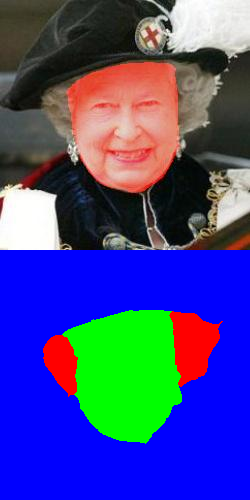
\includegraphics[width=.2\linewidth]{LFW_Presentation/skinProblem_1.png}}}
		\subfloat[Face and skin have same label $\rightarrow$ False negatives]{\makebox[3.5cm][c]{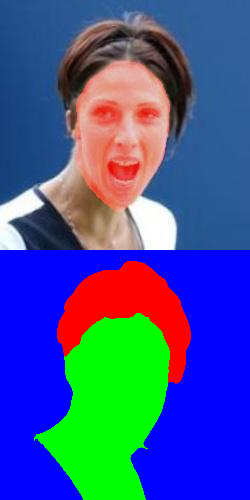
\includegraphics[width=.2\linewidth]{LFW_Presentation/skinProblem_2.png}}}
		\subfloat[Facial hair is an occlusion $\rightarrow$ false positives (hair)]{\makebox[3.5cm][c]{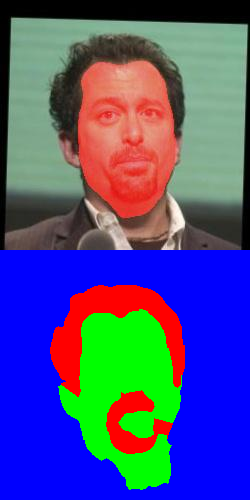
\includegraphics[width=.2\linewidth]{LFW_Presentation/skinProblem_3.png}}}
	\end{figure}
\end{frame}

\begin{frame}[c]{Evaluation on the Parts-LFW Dataset (2)}
	\begin{itemize}
		\item statistics with simple pixelwise comparison
		\item same label for skin parts and face (false negatives)
	\end{itemize}
		\centering
		\begin{figure}
			\begin{center}
				\begin{tabular}{l|l} \hline
					false-positives (hair) & 7.04\%\\ \hline
					false-positives (background) & 0.68\%\\ \hline
					false-negatives (background) & 14.13\%\\ \hline
					right-segmentations & 85.87\%\\ \hline
					right non-sementations & 99.32\% \\ \hline
				\end{tabular}
			\end{center}
		\end{figure}
\end{frame}


\begin{frame}[c]{Evaluation on Synthetic Data (1)}
	\begin{columns}
		\column{.6\textwidth}
		\begin{itemize}
			\item Known ground truth labels (c)
			\item Control of every rotation
			\item Control of the occluded amount
		\end{itemize}
		\column{.28\textwidth}
			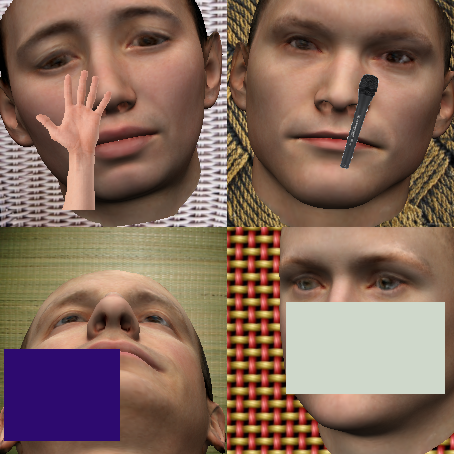
\includegraphics[width=\linewidth]{occlusionTypes/example.png}
	\end{columns}
	\vspace{-1em}
	\begin{figure}
		\centering
		\subfloat[A synthetic face]{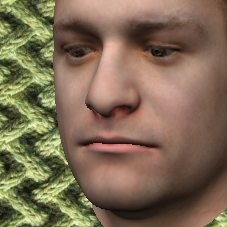
\includegraphics[width=.3\linewidth]{LFW_Presentation/synFace_original.png}}\quad
		\subfloat[A synthetic face with an occlusion]{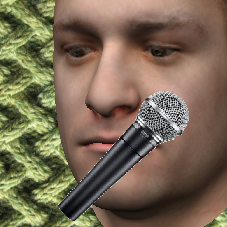
\includegraphics[width=.3\linewidth]{LFW_Presentation/synFace_occluded.png}}\quad
		\subfloat[The ground truth mask of (b)]{\fbox{
\includegraphics[width=.3\linewidth]{LFW_Presentation/synFace_mask.png}}}
	\end{figure}
\end{frame}

\begin{frame}[c]{Evaluation on Synthetic Data (2)}
	\begin{itemize}
		\item Segmentation is very sensitive to the roll rotation
		\item Pitch is asymmetric (better recognizable with high angles)
		\item Yaw rotation has little effect on the segmentation
	\end{itemize}
	\vspace{-1.5em}
	\begin{figure}
		\hspace*{-.8cm}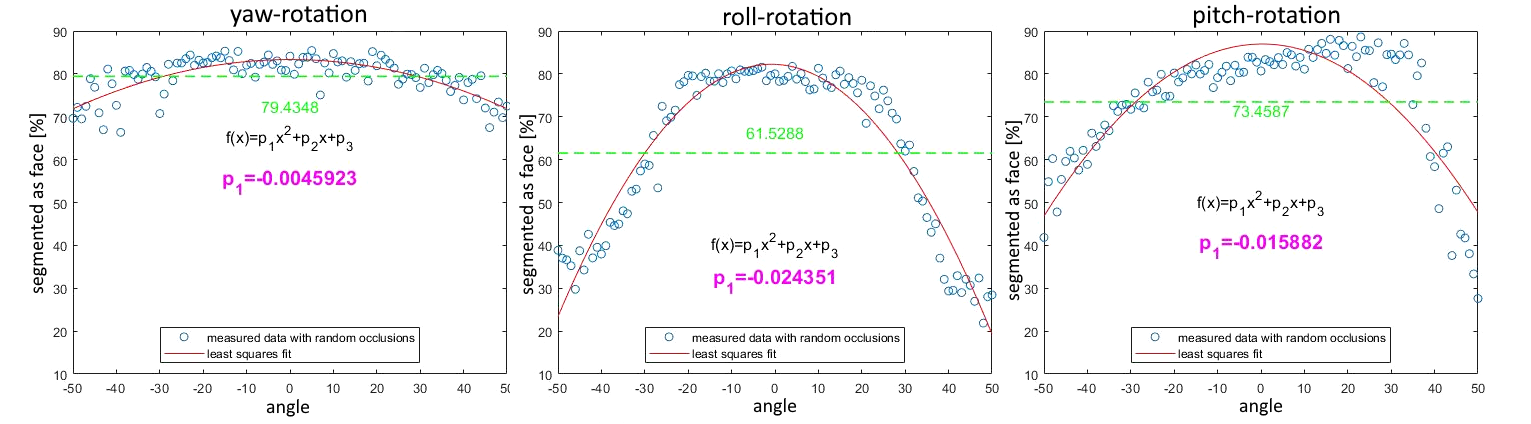
\includegraphics[width=1.15\textwidth]{evaluation_angles.png}
		\caption{Plot for every rotation (yaw, roll, pitch). Quadratic fit (red curve/$f(x)$). Average (green). The data for the plot consisted of synthetic facial images with microphones and hands as occlusions.}
	\end{figure}
\end{frame}


\begin{frame}[c]{Overview}
	\begin{itemize}
		\item \texttransparent{0.4}{Motivation}
		\item \texttransparent{0.4}{Occlusion Segmenation with an FCN}
		\item \texttransparent{0.4}{Experiment: Segmentation Quality}
		\begin{itemize}
			\item \texttransparent{0.4}{Qualitative segmenation results}
			\item \texttransparent{0.4}{Quantitative segmentation results}
		\end{itemize}
		\item Experiment: Fitting under occlusion
		\item \texttransparent{0.4}{Comparison of different approaches}
		\item \texttransparent{0.4}{Future Work}
	\end{itemize}
\end{frame}

\begin{frame}[c]{Fitting with the FCN segmentation (1)}
	\begin{figure}
		\centering
		\subfloat{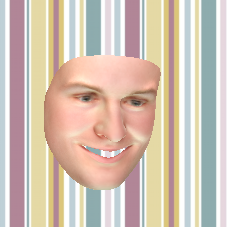
\includegraphics[width=.2\linewidth]{chap3_setting1/hands_setting1_original_test6.png}}\quad
		\subfloat{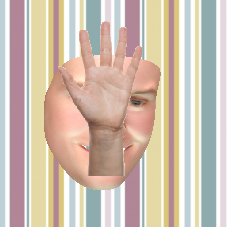
\includegraphics[width=.2\linewidth]{chap3_setting1/hands_setting1_occluded_test6.png}}
	\end{figure}
	\vspace{-1em}
	\begin{figure}
		\newcolumntype{C}{>{\centering\arraybackslash} m{1.7cm} }  %# New column type
		\begin{tabular}{m{1.3cm}|SC|SC|SC|SC}
			& \parbox{2cm}{ground truth mask}& Egger & FCN & no mask\\ \hline
			z-labels & \subfloat{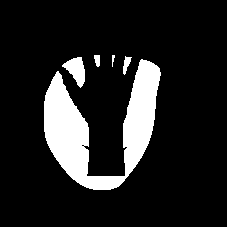
\includegraphics[width=0.1\textwidth]{chap3_setting1/hands_test6_mask_GROTRU.png}} &
			\subfloat{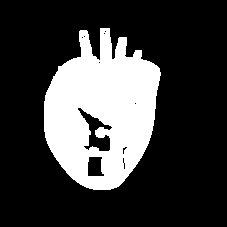
\includegraphics[width=0.1\textwidth]{chap3_setting1/hands_test6_mask_EGGER.png}} &
			\subfloat{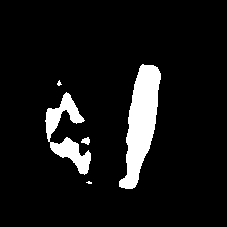
\includegraphics[width=0.1\textwidth]{chap3_setting1/hands_test6_mask_FCN.png}} & \\ \hline
			fits & \subfloat{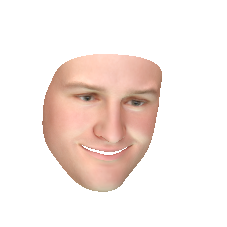
\includegraphics[width=0.15\textwidth]{chap3_setting1/hands_test6_fit_GROTRU.png}} &
			\subfloat{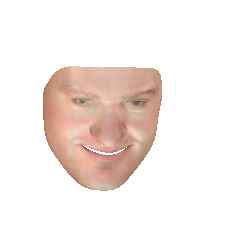
\includegraphics[width=0.15\textwidth]{chap3_setting1/hands_test6_fit_EGGER.png}} &
			\subfloat{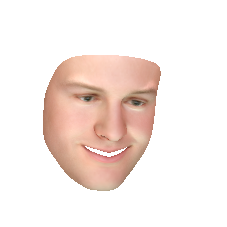
\includegraphics[width=0.15\textwidth]{chap3_setting1/hands_test6_fit_FCN.png}} &
			\subfloat{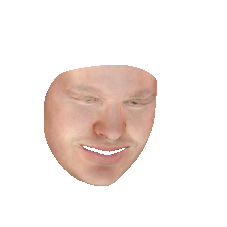
\includegraphics[width=0.15\textwidth]{chap3_setting1/hands_test6_fit_DUMMY.png}} \\
		\end{tabular}
	\end{figure}
\end{frame}

% Tendency decreasing, but increase of the errordue to compensation
\begin{frame}[c]{Fitting with the FCN segmentation (2)}
	\begin{itemize}
		\item Calculation of the error (in $\sigma$) in each iteration
		\item In each parameter-space, we used 50 dimensions
		\item Average over 10 images (only with hands as occlusions)
		\item In each iteration, 1000 samples were drawn
	\end{itemize}
	\begin{figure}
		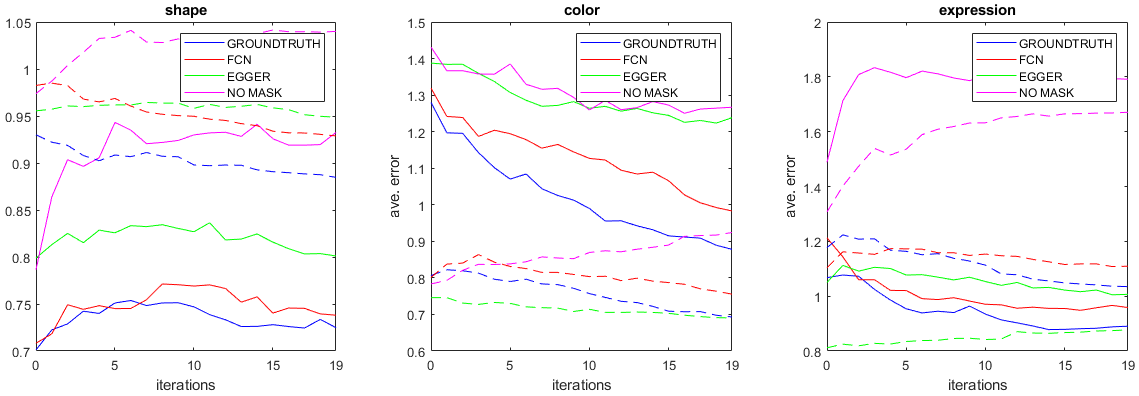
\includegraphics[width=1\textwidth]{chap3_setting1/plot_hands_setting1.png}
		\caption{The average error of the first five (most important) 3DMM parameters is shown with a solid line. The average other 45 parameters is shown with a dashed line.}
	\end{figure}
\end{frame}

\begin{frame}[c]{Oversegmentaion of EGGER}
	\begin{figure}
		\centering
		\subfloat{\fbox{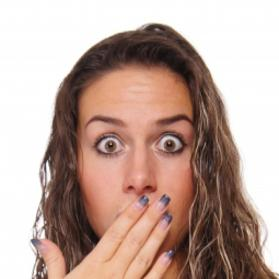
\includegraphics[width=.26\linewidth]{example/original.png}}}\qquad
		\subfloat{\fbox{
\includegraphics[width=.26\linewidth]{example/EGGER.png}}}\qquad
		\subfloat{\fbox{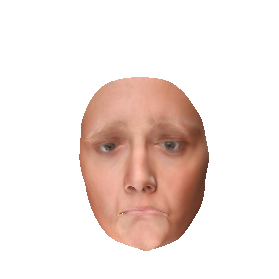
\includegraphics[width=.26\linewidth]{example/fit_EGGER.png}}}\\[.1em]
		
		\subfloat{\fbox{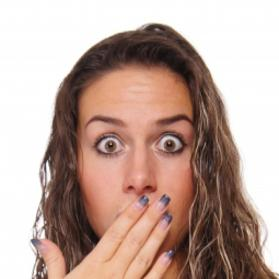
\includegraphics[width=.26\linewidth]{example/original.png}}}\qquad
		\subfloat{\fbox{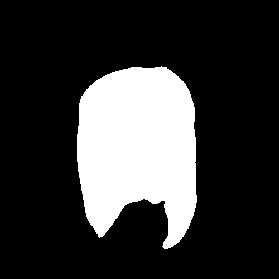
\includegraphics[width=.26\linewidth]{example/FCN.png}}}\qquad
		\subfloat{\fbox{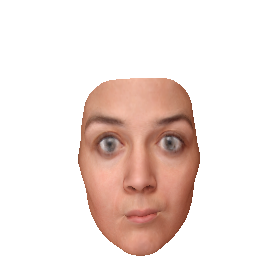
\includegraphics[width=.26\linewidth]{example/fit_GROTRU.png}}}
		
		\caption{Fitting with occlusion-aware masks. Mask of Egger et al (top row). Mask of the fully convolution network used in this thesis (bottom row). }
		\label{fig:3}
	\end{figure}
\end{frame}

\begin{frame}[c]{Fitting with the FCN segmentation (3)}
	\begin{itemize}
		\item Biggest weakness of Egger et al's approach: Oversegmentation
		\item How can we spread between (FCN and EGGER) bigger?
		\item Synthetic faces with both, the 'face12' and the 'bfm' version
	\end{itemize}
	
	\begin{figure}
		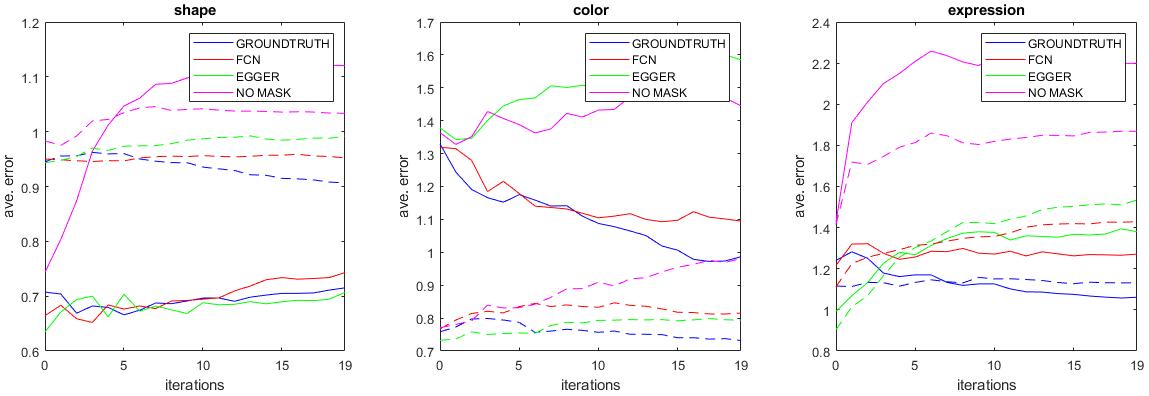
\includegraphics[width=1.05\textwidth]{chap3_setting2/plot_hands_setting2.png}
	\end{figure}
\end{frame}

%\begin{frame}[c]{Runtime (Wall-Clock Time)}
%	\begin{figure}
%		\begin{center}
%			\begin{tikzpicture} 
%			\begin{axis}[ 
%			ybar, 
%			enlargelimits=0.2, 
%			legend style={at={(0.5,-0.15)}, anchor=north,legend columns=-1}, 
%			ylabel={time in [s]}, 
%			symbolic x coords={hands, micros, glasses, no occlusion}, 
%			xtick=data, 
%			ymax=4100,
%			nodes near coords,
%			every node near coord/.append style={rotate=90, anchor=west},
%			] 
%			
%			\addplot coordinates {(hands,3220.89) (micros,1365.68) (glasses,1361.61) (no occlusion,1493.03)}; 
%			\addplot coordinates {(hands,3457.30) (micros,1529.80) (glasses,1491.20) (no occlusion,1499.37)};
%			\addplot coordinates {(hands,3597.28) (micros,1596.89) (glasses,1658.00) (no occlusion,1544.78)};
%			\addplot coordinates {(hands,3476.42) (micros,1506.72) (glasses,1507.20) (no occlusion,1530.41)};
%			
%			
%			\legend{no mask, FCN, Egger et al, ground truth mask} 
%			\end{axis} 
%			\end{tikzpicture}
%		\end{center}
%	\end{figure}
%\end{frame}

\begin{frame}[c]{Overview}
	\begin{itemize}
		\item \texttransparent{0.4}{Motivation}
		\item \texttransparent{0.4}{Occlusion Segmenation with an FCN}
		\item \texttransparent{0.4}{Experiment: Segmentation Quality}
		\begin{itemize}
			\item \texttransparent{0.4}{Qualitative segmenation results}
			\item \texttransparent{0.4}{Quantitative segmentation results}
		\end{itemize}
		\item \texttransparent{0.4}{Experiment: Fitting under occlusion}
		\item Application to real-life data and conclusion
		\item \texttransparent{0.4}{Future Work}
	\end{itemize}
\end{frame}


\begin{frame}[c]{Real-Life data}
	\begin{table}[h!]
		\centering
		\noindent\begin{tabular}{ | m{1.8cm} | m{1.8cm} | m{1.8cm}| m{1.8cm} | m{1.8cm} |}
			\hline
			 & \multicolumn{2}{c|}{\bfseries masks} & \multicolumn{2}{c|}{\bfseries fits} \\ \hline
			original & EGGER & FCN & EGGER & FCN\\ \hline
			
			\begin{minipage}{1.8cm}
				\centering
				\vspace{1pt}
				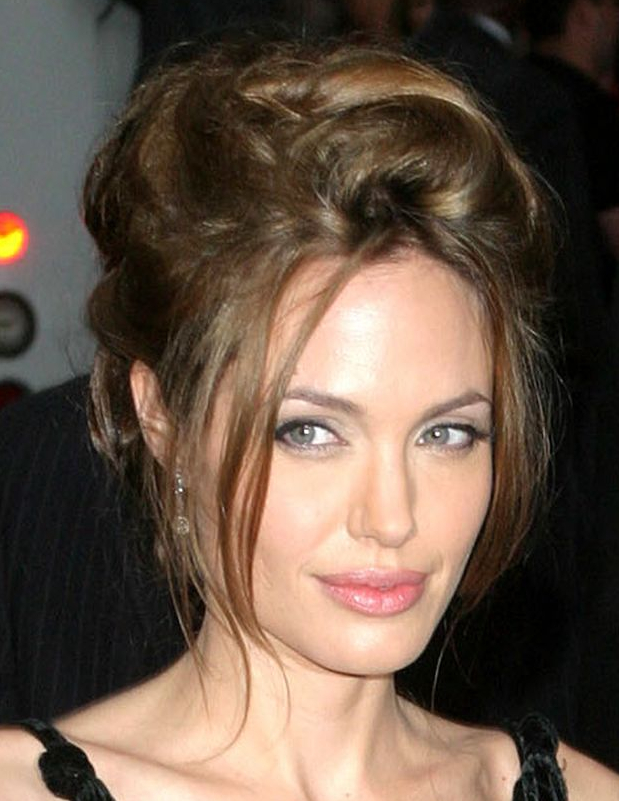
\includegraphics[width=\linewidth]{realLife/test0.png}
				\vspace{1pt}
			\end{minipage}
			&
			\begin{minipage}{1.8cm}
				\centering
				\vspace{1pt}
				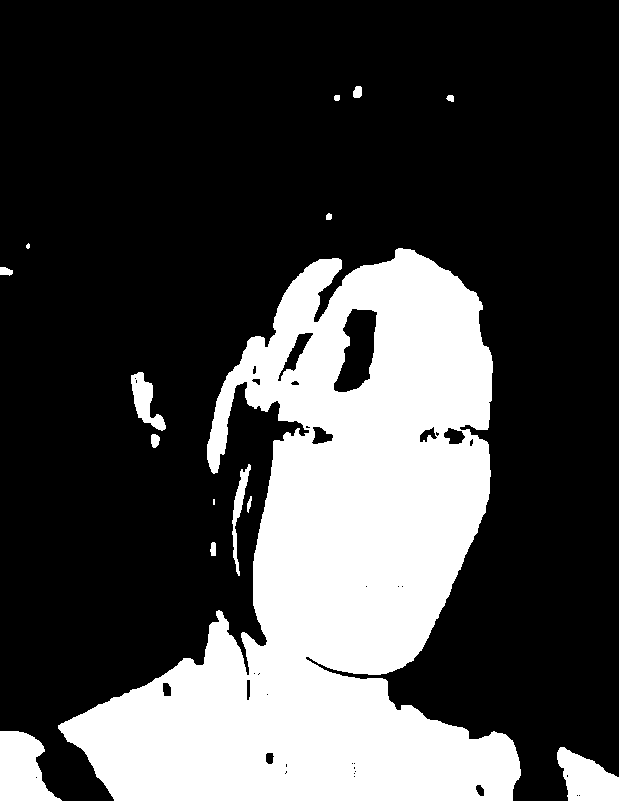
\includegraphics[width=\linewidth]{realLife/test0_mask_EGGER_.png}
				\vspace{1pt}
			\end{minipage}
			& 
			\begin{minipage}{1.8cm}
				\centering
				\vspace{1pt}
				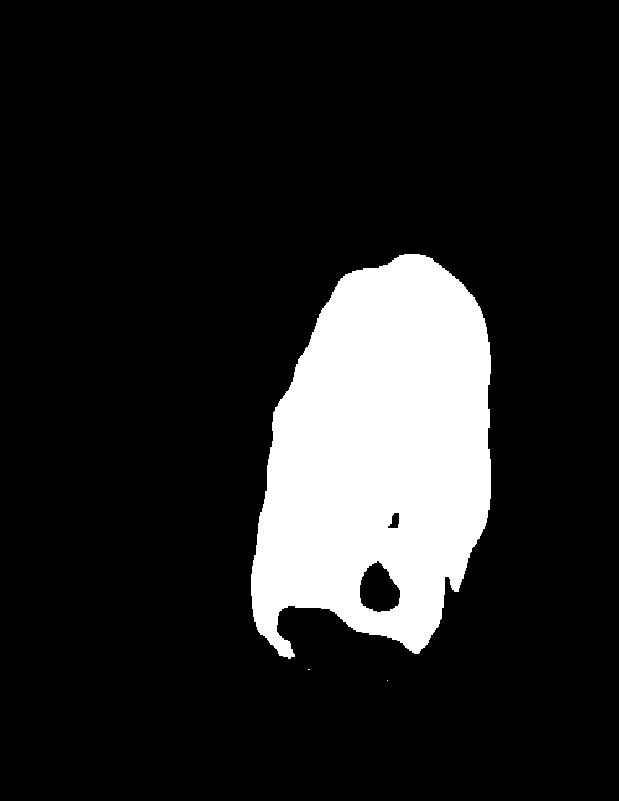
\includegraphics[width=\linewidth]{realLife/test0_mask_FCN_.png}
				\vspace{1pt}
			\end{minipage}
			& 
			\begin{minipage}{1.8cm}
				\centering
				\vspace{1pt}
				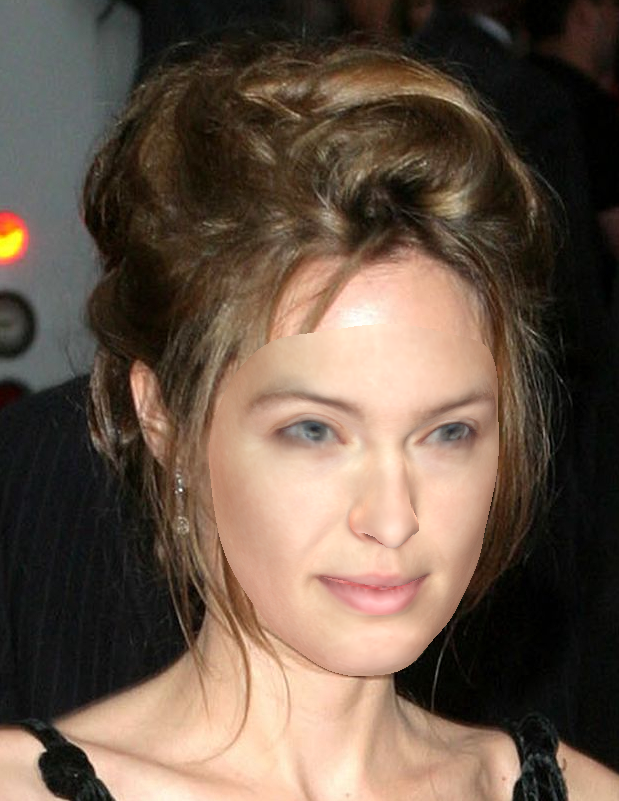
\includegraphics[width=\linewidth]{realLife/test0_overlay_EGGER.png}
				\vspace{1pt}
			\end{minipage}
			& 
			\begin{minipage}{1.8cm}
				\centering
				\vspace{1pt}
				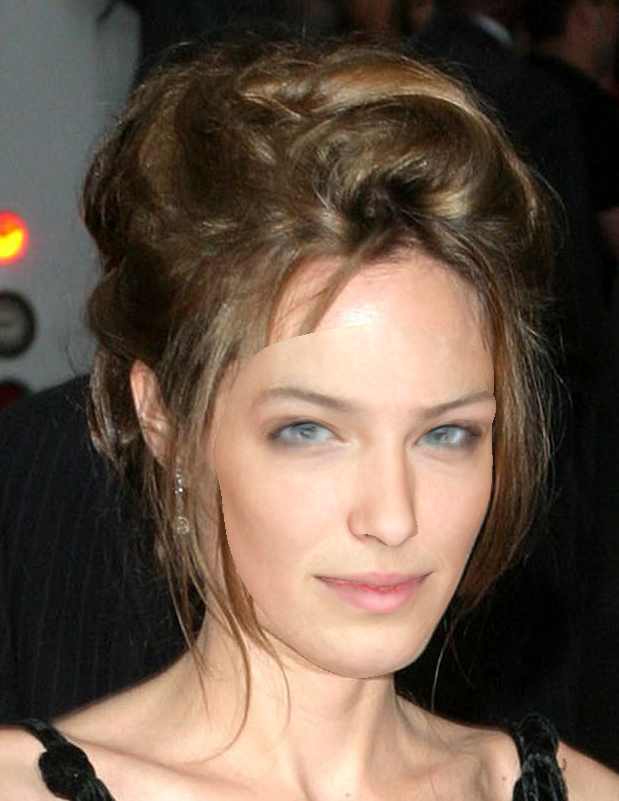
\includegraphics[width=\linewidth]{realLife/test0_overlay_FCN.png}
				\vspace{1pt}
			\end{minipage} \\ \hline
			
			% Here comes the data for the second row
%			
%			\begin{minipage}{1.8cm}
%				\centering
%				\vspace{1pt}
%				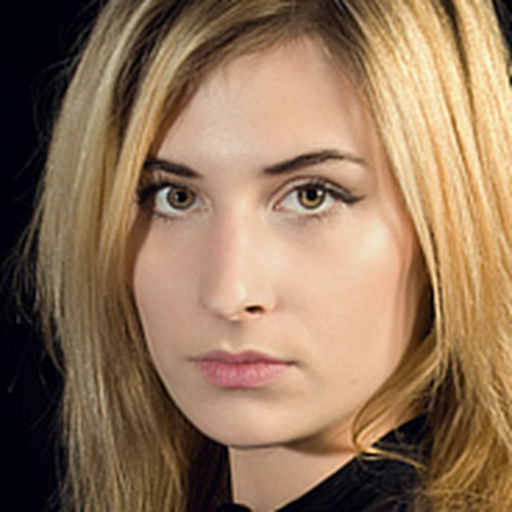
\includegraphics[width=\linewidth]{realLife/test11.png}
%				\vspace{1pt}
%			\end{minipage}
%			&
%			\begin{minipage}{1.8cm}
%				\centering
%				\vspace{1pt}
%				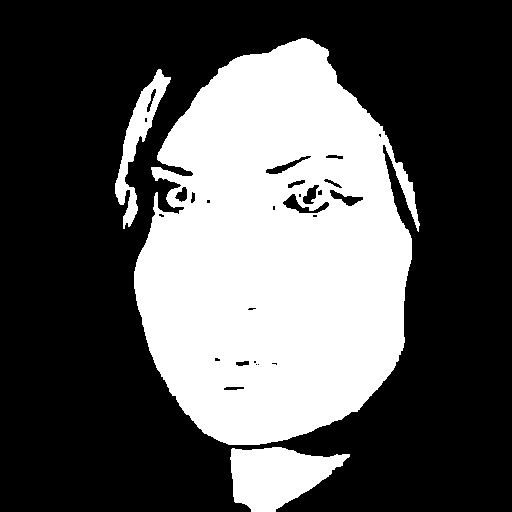
\includegraphics[width=\linewidth]{realLife/test11_mask_EGGER_.png}
%				\vspace{1pt}
%			\end{minipage}
%			& 
%			\begin{minipage}{1.8cm}
%				\centering
%				\vspace{1pt}
%				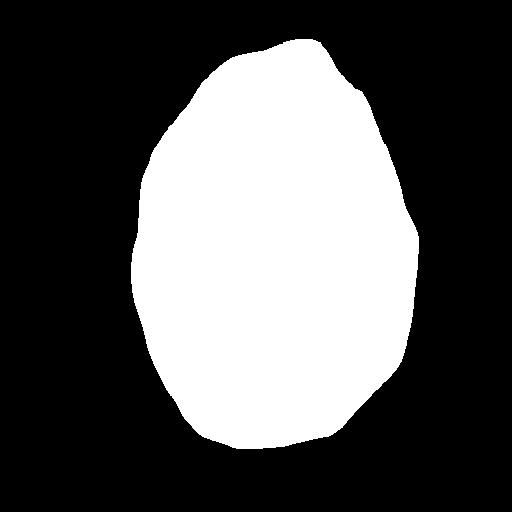
\includegraphics[width=\linewidth]{realLife/test11_mask_FCN_.png}
%				\vspace{1pt}
%			\end{minipage}
%			& 
%			\begin{minipage}{1.8cm}
%				\centering
%				\vspace{1pt}
%				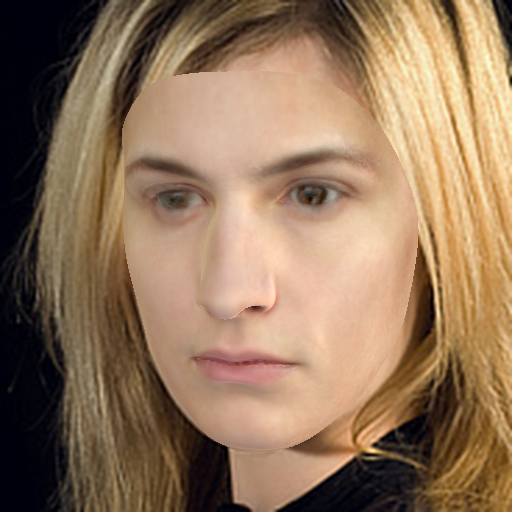
\includegraphics[width=\linewidth]{realLife/test11_overlay_EGGER.png}
%				\vspace{1pt}
%			\end{minipage}
%			& 
%			\begin{minipage}{1.8cm}
%				\centering
%				\vspace{1pt}
%				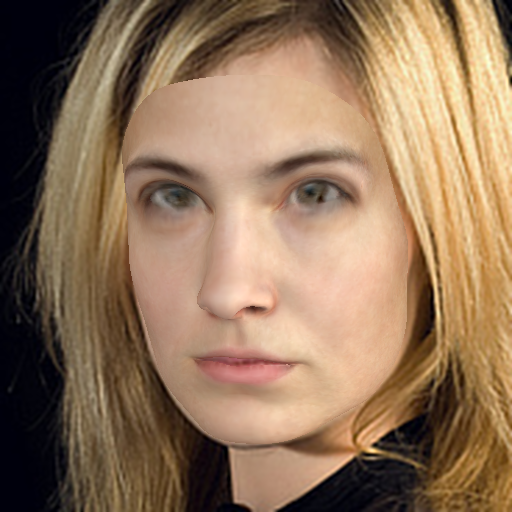
\includegraphics[width=\linewidth]{realLife/test11_overlay_FCN.png}
%				\vspace{1pt}
%			\end{minipage} \\ \hline 
			
			% Here comes the data for the third row
			
			\begin{minipage}{1.8cm}
				\centering
				\vspace{1pt}
				\includegraphics[width=\linewidth]{realLife/test8.png}
				\vspace{1pt}
			\end{minipage}
			&
			\begin{minipage}{1.8cm}
				\centering
				\vspace{1pt}
				\includegraphics[width=\linewidth]{realLife/test8_mask_EGGER_.png}
				\vspace{1pt}
			\end{minipage}
			& 
			\begin{minipage}{1.8cm}
				\centering
				\vspace{1pt}
				\includegraphics[width=\linewidth]{realLife/test8_mask_FCN_.png}
				\vspace{1pt}
			\end{minipage}
			& 
			\begin{minipage}{1.8cm}
				\centering
				\vspace{1pt}
				\includegraphics[width=\linewidth]{realLife/test8_overlay_EGGER.png}
				\vspace{1pt}
			\end{minipage}
			& 
			\begin{minipage}{1.8cm}
				\centering
				\vspace{1pt}
				\includegraphics[width=\linewidth]{realLife/test8_overlay_FCN.png}
				\vspace{1pt}
			\end{minipage} \\ \hline
		\end{tabular}
	\end{table}
\end{frame}

\note{Notes can help you to remember important information. Turn on the notes option.}

\begin{frame}[fragile]{Conclusion}
	\begin{footnotesize}
	\newcolumntype{C}[1]{>{\centering\arraybackslash}m{#1}}
	\begin{tabular}{ r|C{4.15cm}|C{4.15cm} } 
		& \centering advantages & disadvantages \\ \hline
		FCN
		& \onslide<1-4>\begin{itemize}
			\item Does not oversegment
			\item Segments only facepixels
			\item Detects known occlusions
		\end{itemize}
		& \onslide<2-4>\begin{itemize}
			\item Poor detection of thin and new occlusions
			\item Fitting not much faster
			\item Very sensitive to the rotation of the face
		\end{itemize} \\ \hline
		
		\onslide<3->
		EGGER &
		\onslide<3-4>
		\begin{itemize}
			\item Looks at each pixel individually, therefore can detect any occlusion
			\item Stable on real-life data
		\end{itemize}
		& \onslide<4>\begin{itemize}
				\item oversegments
				\item excludes important details on the mask
				\item computes the mask iteratively
			\end{itemize} \onslide<3-> \\ \hline
	\end{tabular}
	\end{footnotesize}
	
	\only<5->{
	\begin{tikzpicture}[overlay]
		\draw [<->, thick, red] (5.45,1.95) to (6.65,3.8);
		\draw [<->, thick, red] (5.45,3.8) to (6.65,1.95);
	\end{tikzpicture}
	}
\end{frame}
	

	%	\begin{columns}
	%		\column{.5\textwidth}
	%		\textbf{Strenghts of the FCN}
	%		\begin{itemize}
	%			\item Does not oversegment
	%			\item Segments almost only facepixels
	%			\item Detects occlusions for which it has been trained
	%		\end{itemize}
	%		\column{.5\textwidth}
	%		\textbf{Weaknesses of the FCN}
	%		\begin{itemize}
	%			\item Performs bad on new occlusions
	%			\item Fitting is not significantly faster
	%			\item Segmentation depends strongly on the rotation of the face
	%		\end{itemize}
	%	\end{columns}
	%	
	%	\begin{columns}
	%		\column{.5\textwidth}
	%		\textbf{Strenghts of the FCN}
	%		\begin{itemize}
	%			\item Does not oversegment
	%			\item Segments almost only facepixels
	%			\item Detects occlusions for which it has been trained
	%		\end{itemize}
	%		\column{.5\textwidth}
	%		\textbf{Weaknesses of the FCN}
	%		\begin{itemize}
	%			\item Performs bad on new occlusions
	%			\item Fitting is not significantly faster
	%			\item Segmentation depends strongly on the rotation of the face
	%		\end{itemize}
	%	\end{columns}
\begin{frame}[c]{Overview}
	\begin{itemize}
		\item \texttransparent{0.4}{Motivation}
		\item \texttransparent{0.4}{Occlusion Segmenation with an FCN}
		\item \texttransparent{0.4}{Experiment: Segmentation Quality}
		\begin{itemize}
			\item \texttransparent{0.4}{Qualitative segmenation results}
			\item \texttransparent{0.4}{Quantitative segmentation results}
		\end{itemize}
		\item \texttransparent{0.4}{Experiment: Fitting under occlusion}
		\item \texttransparent{0.4}{Application to real-life data and conclusion}
		\item Future Work
	\end{itemize}
\end{frame}

\begin{frame}[c]{Future Work: Combination of both masks}
	\begin{table}[h]
		\centering
		\begin{tabularx}{1\textwidth}{>{\centering\arraybackslash}m{2.5cm}| >{\centering\arraybackslash}m{8.5cm}}
			~ & initial mask $\rightarrow$ fitting iterations $\rightarrow$ final mask \\ \hline
			EGGER &
			\vspace{3pt}
			\begin{tikzpicture} 
			\node[inner sep=0pt] (original) at (0,0)
				{\fbox{\includegraphics[width=.12\textwidth]{futureWork/dummy.png}}};
				
			\node[inner sep=0pt] (end) at (6,0)
				{\includegraphics[width=.12\textwidth]{futureWork/test6_mask_EGGER_.png}};
			
			\draw[thick,decoration={aspect=0.5, segment length=6mm,
				amplitude=.5cm,coil},decorate,arrows = {<[bend]-}] (end) --(original);			
			\end{tikzpicture} \\
			\hline
			%\vspace{-4pt}
     		% Data for the second row
			
			FCN &
			\vspace{3pt}
			\begin{tikzpicture} 
			\node[inner sep=0pt] (original) at (0,0)
			{\includegraphics[width=.12\textwidth]{futureWork/test6_mask_FCN.png}};
			
			\node[inner sep=0pt] (end) at (6,0)
			{\includegraphics[width=.12\textwidth]{futureWork/test6_mask_FCN.png}};
			
			\draw [thick,->] (original) edge (end);		
			\end{tikzpicture} \\ \hline
			
			% Data for the third row
			
			Our Combination &
			\vspace{3pt}
			\begin{tikzpicture} 
			\node[inner sep=0pt] (original) at (0,0)
			{\includegraphics[width=.12\textwidth]{futureWork/test6_mask_FCN.png}};
			
			\node[inner sep=0pt] (end) at (6,0)
			{\includegraphics[width=.12\textwidth]{futureWork/test6_mask_combined.png}};
			
			\draw[thick,decoration={aspect=0.5, segment length=6mm,
				amplitude=.5cm,coil},decorate,arrows = {<[bend]-}] (end)--(original);			
			\end{tikzpicture} \\ \hline
			
			% Data for the third row
			
			Future Work &
			\vspace{3pt}
			\begin{tikzpicture} 
			\node[inner sep=0pt] (original) at (0,0)
			{\includegraphics[width=.12\textwidth]{futureWork/test6_mask_FCN.png}};
			
			\node[inner sep=0pt] (end) at (6,0)
			{\includegraphics[width=.12\textwidth]{futureWork/questionmark.png}};
			
			\draw [thick,->] (original) edge (3,0);
			
			\draw[thick,decoration={aspect=0.5, segment length=6mm,
				amplitude=.5cm,coil},decorate,arrows = {<[bend]-}] (end)--(3,0);			
			\end{tikzpicture} \\ \hline
		\end{tabularx}
	\end{table}
\end{frame}

%\begin{frame}[fragile]{Conclusion}
%	\begin{figure}
%		\begin{center}
%			\newcolumntype{C}[1]{>{\centering\arraybackslash}m{#1}}
%			\begin{tabular}{ c C{7cm} } 
%				\textcolor{red}{\textbf{General statement}} & 
%				\begin{itemize}
%					\item \textcolor{red}{Good segmentation under controlled conditions.}
%					\item \textcolor{red}{However, Egger et al's semantic top-down approach is better when there is uncertainty in the data.}
%				\end{itemize}
%			\end{tabular}
%		\end{center}
%	\end{figure}
%\end{frame}

\begin{frame}[t,plain]
\lastpage{{\usebeamerfont{title} Questions?}\\[5ex]
elias.arnold@stud.unibas.ch}
\end{frame}

\note{Notes can help you to remember important information. Turn on the notes option.}

\backupbegin

\begin{frame}[c]{Dependence of the Degree of Occlusion}
	\begin{figure}
		\includegraphics[width=1.0\textwidth]{occVal_angle/occVal_angles_90.png}
	\end{figure}
	\vspace{-1em}
	\begin{figure}
		\begin{center}
			\newcolumntype{C}{>{\centering\arraybackslash} m{
					1.5cm} }  %# New column type
			\begin{tabular}{m{1cm}|SC|SC|SC}
				& yaw & roll & pitch\\ \hline
				-40\textdegree & \subfloat{\includegraphics[width=0.1\textwidth]{asdf/-40_0_0_occVal_20.png}} &
				\subfloat{\includegraphics[width=0.1\textwidth]{asdf/0_0_-40_occVal_20.png}} &
				\subfloat{\includegraphics[width=0.1\textwidth]{asdf/0_-40_0_occVal_20.png}} \\ \hline
				40\textdegree & \subfloat{\includegraphics[width=0.1\textwidth]{asdf/40_0_0_occVal_20.png}} &
				\subfloat{\includegraphics[width=0.1\textwidth]{asdf/0_0_40_occVal_20.png}} &
				\subfloat{\includegraphics[width=0.1\textwidth]{asdf/0_40_0_occVal_20.png}} \\
			\end{tabular}
		\end{center}
	\end{figure}
\end{frame}


\begin{frame}[c]{Wrong Color Choice with the Mask of Egger et al}
	\vspace{-1em}
	\begin{tikzpicture}
	\node[inner sep=0pt] (original) at (0,0)
	{\includegraphics[width=.25\textwidth]{chap3_setting2/hands_setting2_test0.png}};
	
	\node[inner sep=0pt] (fcn_mask) at (4.5,1.7)
	{\includegraphics[width=1.5cm]{chap3_setting2/hands_test0_mask_FCN_.png}};
	\node[inner sep=0pt] (egger_mask) at (4.5,0)
	{\includegraphics[width=1.5cm]{chap3_setting2/hands_test0_mask_EGGER_.png}};
	\node[inner sep=0pt] (groundtruth_mask) at (4.5,-1.7)
	{\includegraphics[width=1.5cm]{chap3_setting2/hands_test0_mask_GROTRU_.png}};
	
	\node[inner sep=0pt] (fcn_fit) at (9,1.7)
	{\includegraphics[width=2cm]{chap3_setting2/hands_test0_fit_FCN.png}};
	\node[inner sep=0pt] (egger_fit) at (9,0)
	{\includegraphics[width=2cm]{chap3_setting2/hands_test0_fit_EGGER.png}};
	\node[inner sep=0pt] (groundtruth_fit) at (9,-1.7)
	{\includegraphics[width=2cm]{chap3_setting2/hands_test0_fit_GROTRU.png}};
	
	
	\path[every node/.style={font=\sffamily\small}]
	
	([yshift=-5pt] original.north east) edge [out=0,in=180,->]node [above=3pt] {FCN} (fcn_mask)
	
	(original) edge [out=0,in=180,->]node [above=3pt] {EGGER} (egger_mask)
	
	([yshift=5pt] original.south east) edge [out=0,in=180,->]node [below=3pt,xshift=-.5cm,yshift=-.1cm] {GROUNDTRUTH} (groundtruth_mask)
	
	(fcn_mask) edge [out=0,in=180,->]node [above=3pt] {} (fcn_fit)
	
	(egger_mask) edge [out=0,in=180,->]node [above=3pt] {} (egger_fit)
	
	(groundtruth_mask) edge [out=0,in=180,->]node [above=3pt] {} (groundtruth_fit);
	
	\end{tikzpicture}
	%\vspace{-2em}
	\begin{tikzpicture}
	\tikzstyle{line} = [draw, -latex']
	
	\node[inner sep=0pt] (egger_vs_fcn) at (0,0)
	{\includegraphics[width=\textwidth]{wrongColor/example.png}};
	
	\path [line,line width=0.5mm,red] (-5.6,-1.5) -- node [text width=2.5cm,above,xshift=.5cm] {EGGER} (-0.2,-1.5);
	
	\path [line,line width=0.5mm,blue] (5.6,-1.5) -- node [text width=2.5cm,above,xshift=.7cm] {FCN} (0.2,-1.5);
	
	\end{tikzpicture}
	%\vspace{-2em}
\end{frame}

\begin{frame}[c]{Related Work (Nirkin et al: On Face Segmentation, Face Swapping, and Face Perception)}
	\begin{itemize}
		\item Widespread artificial neural networks can be used for  face segmentation
		\item intra-subject swapped faces remain as recognizable as their sources (a)
		\item less recognizable inter-subject results (b)
	\end{itemize}
	\begin{figure}
		\centering
		\subfloat[Example of Intra-Subject swapping]{\includegraphics[width=.48\linewidth]{Bilder_Praesentation/Inter.JPG}}\quad
		\subfloat[Example of Inter-Subject swapping]{\includegraphics[width=.48\linewidth]{Bilder_Praesentation/Intra.JPG}}
	\end{figure}
\end{frame}

\backupend

\end{document}

